\documentclass{article}
\usepackage[utf8]{inputenc} % Så vi kan rocka på värmländska 
\usepackage[parfill]{parskip}  %För att slippa den där jävla indenteringen
\usepackage{graphicx} % För plottarna
\usepackage{color}  %plottarna
\usepackage{amsmath}
\usepackage{float} % Få plott fan att stanna 
\usepackage[english]{babel} %ingen aning om varför desperat copy paste
\usepackage{url} %för längar 

\title{Player positions in the NBA \\
\large  732A61 Data Mining \\
 Clustering and Association Analysis }
\author{Emil Klasson Svensson
 \\IDA, Statistics and Data Mining
\\Linköping University
\\emisv463@student.liu.se}
\date{June 2017}


\begin{document}

\maketitle
\thispagestyle{empty}
\newpage

\section{Introduction}

Basketball is one of the largest and most popular sports in the world . It is a team sport where two teams fielding five players each trying to put the ball through the opponents’ basket with the team scoring most points being the winning side. One team usually fields different types players according to their given position, this is a position given arbitrary given the players physical appearance. \cite{wikibasket} The goal is to find new positions clustering algorithms given data rather than the traditional approach. The project will focus on analyzing data collected from the National Basket Association (NBA) which is today regarded as the league with has the highest level of professional basketball.
 
This project is loosely based around an paper written by Dwight Lutz called \textit{A Cluster Analysis of NBA Players} \cite{lutz2012cluster} which revolves around finding clusters of NBA-players (basketball players) and giving them a new class-labeled for basketball players positions on court.


%\subsection{What is Basketball?}


\subsection{Positions in Basketball}

Traditionally players are labeled according to the respective task on the court, called positions. In this standard there are five different positions

\begin{enumerate}
\item Center 
\item Power Forward
\item Small Forward
\item Shooting Guard
\item Point Guard
\end{enumerate}

Small and fast players are often referred to as guards (point guard/shooting guard) with main focus on handeling, distributing and scoring. Tall and strong players are labeled (power/small-) forward or center. The small forward task i mainly scoring and grabbing rebounds while Power forward and Center have a bigger role in setting screens for smaller players and grabbing rebounds, there is no formal way of determining what position a player should be according to these five current positions and it is up to coaches to decide this and this affects the way the player on the position play and acts.


In the modern NBA something that is called “position less basketball” have gained popularity with many coaches moving away from defining their players according to the classic positions and playing different line ups with players which traditionally would play on the same position. \cite{positonbasketball} This trend has led to journalists inventing more labels to describe players in order to find some structure.



\subsection{Objective}


The goal with this project will be to via multivariate cluster analysis identify new and more appropriate labels for players defined by their performance on the court rather than traditional perceptions. A qualative and quantative analysis of the clusters and members of the different clusters will be done to evaluate and discuss the quality of the result along with comparison to the result in Dwight Lutz called "A Cluster Analysis of NBA Players".



\section{Variables}

The data collected are from NBAs webpage nba.com using web scraping tools and some pre-processing. The set in total contains 33 different variables from 271 players during the season of 2015-2016 where all variables were aggregated by average per game. Players playing under 40 games were excluded from the data set since only frequently used player are of interest to find belongings to. The decision to only use data from one year instead of over consecutive years was determined by the context of the project. Seeing how the trend of so called possitionless basketball is a relatively new phenomena having data spanning over multiple years might wash away characteristics of averages for players that have been in the league during multiple years. The down side of this is the problem of having to few observations may lead to clusters being hard to define since a lower amount of observations. In the table below all variables used in the clustering are presented.

\begin{table}[ht]
\centering
\begin{tabular}{rll}
  \hline
 & \textbf{Abbrivations} & \textbf{Explanation} \\ 
  \hline
1 & MIN & Minutes played \\ 
  2 & FGA & Field Goals Attempted \\ 
  3 & FG\_PCT & Field Goal Percentage \\ 
  4 & FG3A & 3-Point Field Goals Attempted \\ 
  5 & FG3\_PCT & 3-Point Field Goal Percentage \\ 
  6 & FTA & Free Throws Attempted \\ 
  7 & FT\_PCT & Free Throw Percentage \\ 
  8 & OREB & Offensive rebound \\ 
  9 & DREB & Defensive Rebound \\ 
  10 & AST & Assist \\ 
  11 & STL & Steals \\ 
  12 & BLK & Blocked shot \\ 
  13 & TOV & Turnovers \\ 
  14 & PTS & Points Made \\ 
  15 & DistFeet & Distance coverd in feet \\ 
  16 & AvgSpeed & Average Speed \\
   \hline
\end{tabular}
\caption{\textit{Variables used in clustering and visualisation}} 
\end{table}

In the original collected dataset each player had 31 different variables (excluding player names and player ID) available in Appendix A. All of these variables are aggregated as the average of games played. Many of the original variables are naturally connected and correlated as for example Field Goal - Percentage (FG\_PCT) is a function of the variables Field Goals Made, Field Goals Attempted. So in order to try to reduce the number of dimensions in the dataset but still keep information variables that describes Made - Fields Goals, 3 Point Field Goals and Free Throws were removed since they are described in their respective percentages, although this is true for the number of attempts it is an interesting variable since that players taking shots indicates some sort of action on court compared to the act of making a shot which is just one of two consequences of shooting the ball. The variable EFF was also removed since it is a function of several of the other variables and doesn't describe any action on the court. Other than that all variables removed were removed because they are a superset or subset of each other.

All variables were standardized before clustering in the following manner to give each variable the same weight.

 $$z_{ij} = \frac{x_{ij} - \mu_{j}}{\sigma_{j}}$$ 

Later in the report the unstandardized variables are presented along with the cluster labels in order to help the readers get a more interpretable result.

%Nagat skrap eller mening som kanske ar bra senare.
%Since this project aims to identify and find different types of players as many defining characteristics were preferred as well defined 

\newpage


\section{Method}

\subsection{t-SNE}


t distributed Stochastic Neighborhood Embedding (t-SNE) is a dimensionality reduction technique that aim to take a data set with k dimension and project them on to a 2 dimensional or 3 dimensional plane with the goal to display similar objects from the high dimensional data set close to each other in the lower dimensional plane.

It uses conditional probabilities $p_{i|j}$  to model the high dimensional probability of observation $x_i$ picking $x_j$ as its neighbor under a t-distributed kernel. This is then compared to the probability  which is is the same but in the low dimensional space where it tries to project these observations. These distributions are then compared with the Kullback Leibler divergence, this is the algorithms cost function where the high and low dimensions’ match with the same probability reaches its minimum.

$$C = KL(P||Q)=\sum_i\sum_jp_{ij}log(\frac{p_{ij}}{q_{ij}})$$

The minimization technique used is gradient decent which iteratively walks through the space in order to find a local minimum with a selected step size in proportion to the second derivative of the cost function also known as the gradient.

The variance in the kernels are set by the parameter perplexity which i a tunable hyper parameter that tries to catch the relationship between the local and the global structure of the data in order to preserve it in the low dimensional space. According to the authors of the paper the algorithm provides stable results for values between 5 and 50, in this project different perplexity values will be explored and evaluated. \cite{ictdbid:2777}

The implementation used is implemented in R and is from the package "tsne".




\subsection{EM-algorithm}

Expectation-maximization algorithm (EM Algorithm) is a technique that uses the observed data and a latent variable that is the unobserved data and tries to find the maximum likelihood estimation (MLE). It is a general method with many applications in the area of data mining where clustering is one of them.

In this project a mixture of Gaussians will be used due to the fact that it is the only available implementation in R. The package name is mclust. This leads to an assumption that all observations are independently identically normal distributed. This assumption is in this project questionable since there every player on court impacts each other in significate way. But previous result has shown that the normality assumption is fairly robust and are therefore accepted.

All of the observed data points are denoted X and the unobserved (Also called latent variables) points are denoted Z. These two variables are assumed to each have some sort of probability distribution given a unknown parameter $theta$. In the case of clustering the cluster-group is considerd to be unkown and is denoted as the latent variable in this case. Combining these two distributions will give us our joint distribution. From here the algorithm starts iterating through the two steps, the Expectation-step and the second one being the maximization - step.

In the E-step we calculate the probability for each observation in Z belonging too the different cluster labels given the data and a current estimate of this parameter theta that we are updating.


$$\gamma(z_{nk}) = \frac{\pi_k N(x_n|\mathbf{\mu}_k,\mathbf{\Sigma}_k)} {\sum_{j=1}^{K}  \pi_jN(x_n|\mathbf{\mu}_j,\mathbf{\Sigma}_j)}$$

With this information we then move on to the M-step where the probabilities from the E-step are used to compute the weighted averages between the probabilities $Z_{ij}$ for belonging to each cluster multiplied with the observed value $X_{ij}$ to get the cluster centroids.

$$\mathbf{\mu}_k^{new} = \frac{1}{N_k} \sum_{n=1}^N\gamma(z_{nk})x_n$$

$$\mathbf{\Sigma}_k^{new} = \frac{1}{N_k} \sum_{n=1}^N\gamma(z_{nk})(x_n-\mathbf{\mu}_k^{new})(x_n-\mathbf{\mu}_k^{new})^T$$

$$ \pi_k^{new}= \frac{N_k}{N} $$ 
where
$$  N_k = \sum_{n=1}^N \gamma(z_{nk})$$

With the new parameters we evaluate the log of likelihood with these newly updated parameter and check if we have found a stable result, if not, these two steps are repeated back and forth until an stable is found or the max number of iterations is reached. Since the joint likelihood function is almost always multimodal the algorithm is only guaranteed to find a local optimum.

This updating procedure means that the observations are not hard-assigned to one cluster until convergence (via argmax) but instead given a probability to be in each cluster allowing for more dynamical clustering approach to the data in the way that it is able to find different density regions in the data. \cite{Bishop:2006:PRM:1162264}

The cluster size was set to 10 to be able to compare the result with the previously mentioned paper \textit{A Cluster Analysis of NBA Players} \cite{lutz2012cluster}


%Kanske lite om relationen till K-means för att runda upp det hela? 


%With these two parameters we define a joint distribution that we then try to find the maximum likelihood estimated parameters via a expectation and a maximization step.

\newpage

\section{Results}

\subsection{Visualization with t-SNE}

The process of finding a good visualization for t-SNE for this project started out with a sequence of 5 different values from 10 to 50 to try to get a feeling for how the algorithm handled the data. On all levels of perplexity the algorithm seemed to not any noticeable changes in minimizing the cost function after around 1500 iterations. For the perplexity number the lower values of perplexity seem to yield better separation between visually identified clusters. The projections placement in relationship to each other were often time close to each other independent of the perplexity setting. Of the five initial runs values a perplexity of 10 was determined to be the best and values 5 and 15 for perplexity were explored to try to see the general trend of how the projections behaved. When trying a perplexity above 10 the separation seemed to be washing away a bit. For values in the lower range with a perplexity of 5 the separation seems to be increasing but observations were in very small clusters of two to ten players in each cluster. To try to find a good balance between the local and global structure in the projection the final perplexity was set to 10 which is here presented.

\begin{figure}[H]
 \centering
 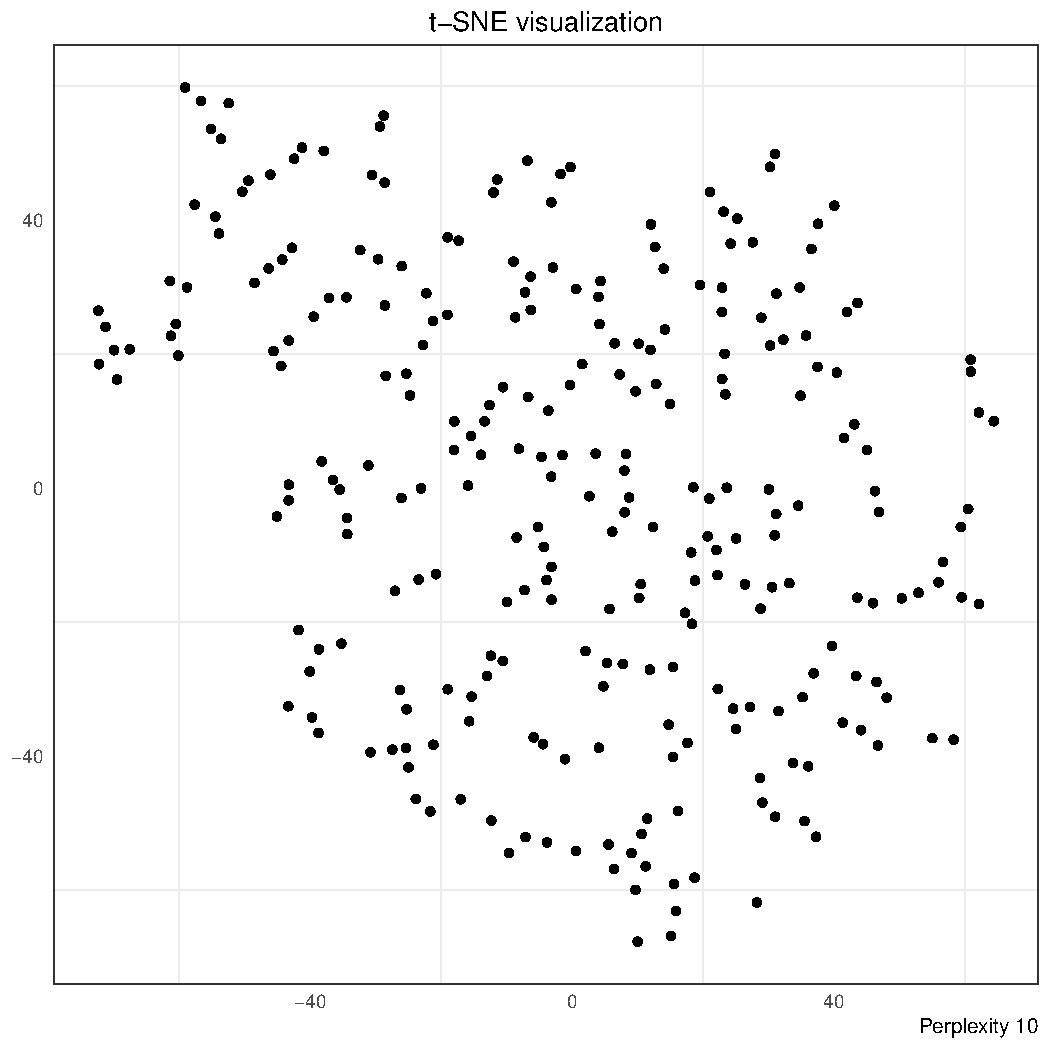
\includegraphics[height=8cm]{tsne10}.
 \caption{t-SNE visualization with perplexity 10}
 \label{figure:1}
\end{figure}

In the graph above a fairly large group consisting of around 30-40 observations that are located in the right corner of the graph. In the middle of the graph a larger amount of observations seems to be scattered around with some observations being closer together and might even be considered clusters. In general observations tend to be smaller sub clusters closer to each other although the large cluster is separated from the other observations. In the bottom right there also seems to be a cluster of points separated from the middle. From the bottom middle leaning towards top left is a oblong shaped point spread that is fairly separated from the middle as well. In the following graph ill zoom in on the cluster in the bottom right frame of the scatterplot to be able to present which players the points represent. Overall the observations in the different clusters look somewhat similar although there are some players that seems to be out of placed compared to its neighbors.

%In the top left there also seem to be an almost oval shaped cluster with players.  The 

%In the lower left corner there seem to be one or two clusters with in total around 20 similar observations.  Above this cluster there seem to be a similar sized cluster. In the bottom middle there also seem to be a cluster that could be divided in to several small clusters. The same goes for what seems to be a cluster in the middle of the graph. In the right side of the graph there seem to be one cluster moving up towards the corner where another cluster appears. Around these two clusters are two "strings" with players that are not a part of the clusters one in the middle top and one in the top right corner.

 
\begin{figure}[H]
 \centering
 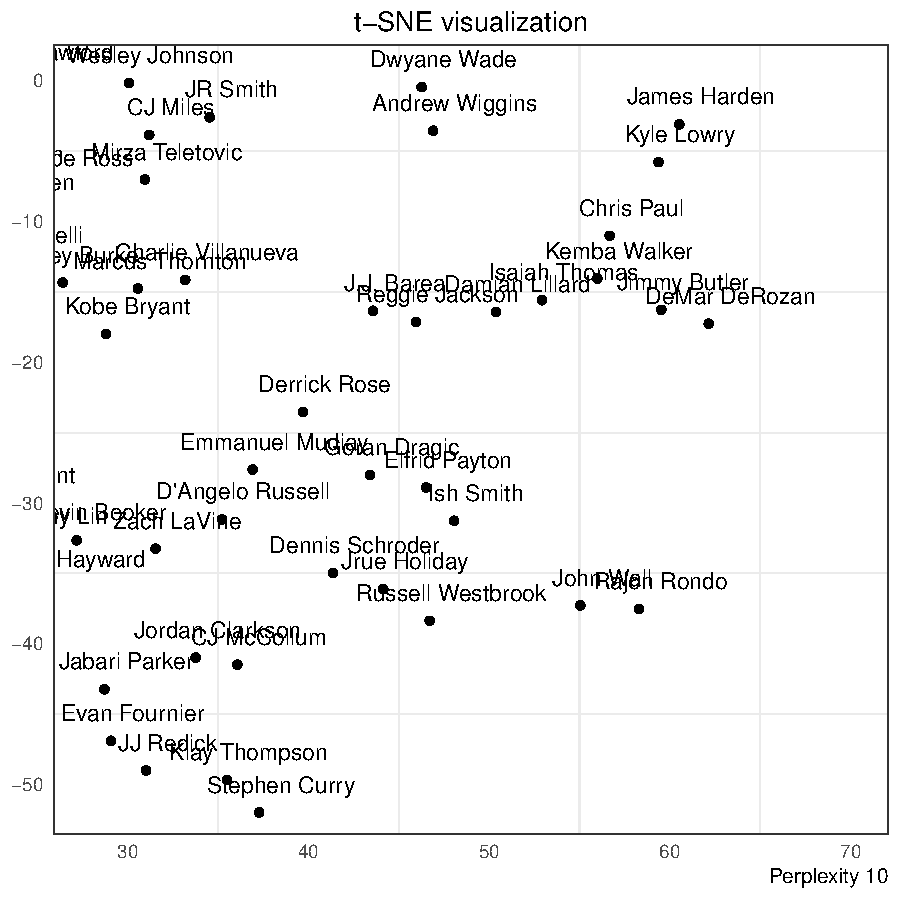
\includegraphics[height=8cm]{zoom10}.
 \caption{t-SNE visualization with perplexity 10 zoomed in}
 \label{figure:2}
\end{figure}

In this part of the graph we can see some of the player and their respective name. This cluster seems to contain players that are normally in the point or shooting guard position. The top part has some player separated from the other that seem together on a horizontally flipped "Y". These players are known for high scoring, lots of assists and holding a fast pace.
 
\newpage 
 
\subsection{Clustering} 

The EM algorithm with 10 clusters converged and below is the unstandardized averages for each cluster presented.

\begin{table}[ht]
\centering
\resizebox{\textwidth}{!}{%
\begin{tabular}{rrrrrrrrr}
  \hline
  Cluster & $n_k$  & FGA & FG\_PCT & FG3A & FG3\_PCT & FTA & FT\_PCT \\ 
  \hline
1 &  22 & 12.91 & 0.44 & 4.29 & 0.33 & 3.00 & 0.81 \\ 
  2  &  37 & 4.85 & 0.46 & 1.41 & 0.37 & 1.14 & 0.72 \\ 
  3 &  35 & 9.93 & 0.43 & 3.91 & 0.35 & 2.45 & 0.78 \\ 
  4  &  24 & 11.55 & 0.53 & 0.89 & 0.21 & 4.25 & 0.70 \\ 
  5  &  19 & 6.26 & 0.48 & 1.90 & 0.26 & 1.53 & 0.69 \\ 
  6  &  24 & 16.63 & 0.45 & 4.90 & 0.35 & 5.92 & 0.82 \\ 
  7  &  18 & 5.68 & 0.39 & 2.97 & 0.33 & 0.78 & 0.83 \\ 
  8  &  30 & 5.18 & 0.52 & 0.10 & 0.07 & 1.72 & 0.69 \\ 
  9  &  41 & 9.02 & 0.44 & 2.80 & 0.34 & 2.09 & 0.78 \\ 
  10  &  21 & 6.50 & 0.44 & 2.31 & 0.34 & 1.65 & 0.74 \\ 
   \hline
\end{tabular}%
}
\caption{EM algorithm 10 cluster result: average shooting stats} 
\end{table}


\begin{table}[h]
\centering
\resizebox{\textwidth}{!}{%
\begin{tabular}{rrrrrrrrrrrr}
  \hline
   Cluster & $n_k$ & MIN & OREB & DREB & AST & STL & BLK & TOV & PTS & DistFeet & AvgSpeed \\ 
  \hline
1 & 22 & 31.59 & 1.26 & 4.60 & 2.12 & 1.01 & 0.43 & 1.59 & 15.41 & 11513.27 & 4.13 \\ 
  2 & 37 & 16.58 & 0.87 & 2.51 & 0.93 & 0.44 & 0.31 & 0.76 & 5.79 & 6193.00 & 4.26 \\ 
  3 &  35 & 28.68 & 0.82 & 3.32 & 2.56 & 1.03 & 0.33 & 1.50 & 11.81 & 10394.37 & 4.11 \\ 
  4 &  24 & 31.20 & 2.65 & 6.84 & 2.10 & 0.92 & 1.63 & 1.91 & 15.15 & 10924.22 & 3.98 \\ 
  5 &  19 & 23.28 & 1.20 & 3.06 & 1.07 & 0.65 & 0.55 & 0.83 & 7.62 & 9045.08 & 4.41 \\ 
  6 &  24 & 34.97 & 0.98 & 4.58 & 5.93 & 1.42 & 0.47 & 2.98 & 21.60 & 12438.65 & 4.03 \\ 
  7 &  18 & 17.60 & 0.41 & 1.91 & 1.17 & 0.53 & 0.21 & 0.71 & 6.04 & 6391.10 & 4.13 \\ 
  8 &  30 & 18.52 & 1.80 & 3.59 & 0.95 & 0.45 & 0.82 & 0.99 & 6.59 & 6635.47 & 4.08 \\ 
  9 &  41 & 26.24 & 0.59 & 2.61 & 3.40 & 0.90 & 0.29 & 1.64 & 10.50 & 10096.41 & 4.37 \\ 
  10 &  21 & 20.81 & 0.62 & 2.36 & 2.13 & 0.87 & 0.26 & 1.18 & 7.77 & 7658.41 & 4.18 \\ 
   \hline
\end{tabular}%
}
\caption{EM algorithm 10 cluster result: averages for non-shooting stats} 
\end{table}



\begin{table}[h]
\centering
\resizebox{\textwidth}{!}{%
\begin{tabular}{lllll}
  \hline
Cluster lables & Cluster & Typical players  &  &  \\ 
  \hline
   Shooting Froward & 1 & Klay Thompson & Kawhi Leonard & CJ McCollum \\ 
  Back Up Forward & 2 & Jonas Jerebko & Leandro Barbosa  & Derrick Williams \\ 
  Versatile Forward & 3 & Jeff Teague & Lou Williams & Jae Crowder \\ 
   Elite Bigs & 4 & Anthony Davis & Brook Lopez & Karl-Anthony Towns \\ 
   Mobile Bigs & 5 & Myles Turner & Steven Adams  & Doug McDermott \\ 
  Elite Scorers & 6 & Stephen Curry & James Harden & Kevin Durant \\ 
  Veterans & 7 & Marcus Thornton & Gerald Green & Wayne Ellington \\ 
  Defensive Bigs & 8 & Robin Lopez & Tim Duncan & Timofey Mozgov \\ 
  Distributors & 9 & Jrue Holiday & Derrick Rose & JJ Redick \\ 
  Stretch Big & 10 & Mirza Teletovic & Kelly Olynyk & Nikola Jokic \\ 
   \hline
\end{tabular}%
}
\caption{Cluster lables and typical players} 
\end{table}

Cluster 1 and 3 are quite similar with distinctions in that player from cluster 1 takes more shots and makes them at a similar percentage in just a bit longer time on the court. Another difference between them seems to be the distance they run, players from cluster 1 run about 1500 feet longer than the players from cluster 3, this is probably mostly attributed by the fact that they play for extended minutes compared to cluster 3. When inspecting the players in the clusters the only difference noticeable is what roles the players have in their respective teams, where most players from cluster 1 have an more offensive role in general and the other ones are more of defensive-minded players and playmakers. Cluster two consists of players that on average preform less in all categories than the previously named clusters but also play less minutes.

The fourth clusters consist of players on average attempting less than one shot outside the three-point line a game with low accuracy. But these players shoot frequently and with good percentage. They also grab a lot of offensive rebounds and averages the most blocked shots among the clusters. They do this while still moving a lot but at a slower pace than other clusters. The player in this cluster are the best big players of the game at the moment and the cluster is therefor called "Elite Bigs". Compared to cluster 4 cluster 5 consists of player with similar features but with less shots attempted and made. The big difference is that they move at a lot higher average speed than in cluster 4 and 8. Cluster 8 shares similar traits to the fourth and fifth clusters but almost never attempt any 3 points shots and when they do its at an low percentage, they also move on average among the least distance of the clusters. When inspecting these cluster these are players who have roles clearly defined as the traditional center position with a bigger role on defense.

The most clear cut cluster is number 6 where basically every variable is above all other cluster, these are players who score at a high rate with good accuracy and overall considered to be their respective teams best players.

The biggest cluster is cluster 9 which consists of players shooting relatively frequently at relatively good percentages, they have the highest number of assists outside cluster 6 and are also moving at a high speed for long distances on average. The players in this cluster are to be considered players distributing the ball and setting plays for other players.

\subsection{EM Clustering with t-SNE visualization}

\begin{figure}[H]
 \centering
 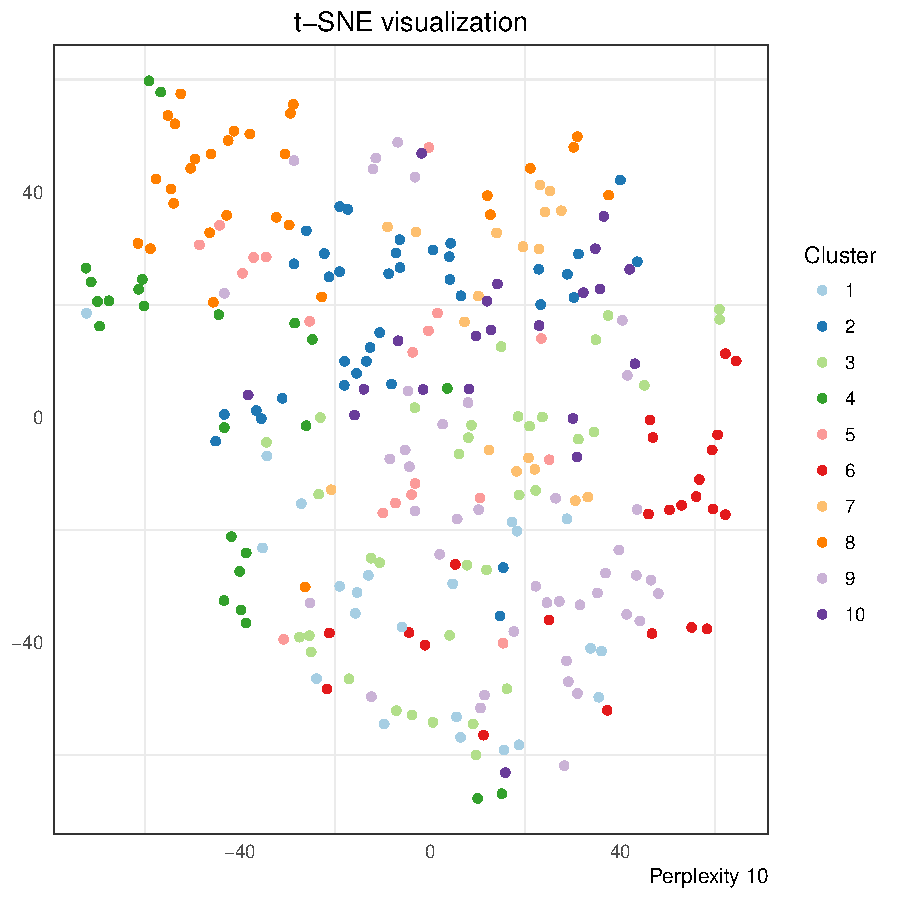
\includegraphics[height=10cm]{tsnecluster2.pdf}.
 \caption{t-SNE visualization with clustering from EM -algorithm}
 \label{figure:2}
\end{figure}

In the middle region the cluster belongings from the EM-algorithm are dispersed and dose not land close to each on the visualization other than small groups of 2-3 players. In the right region of the graph a couple of the players from cluster 6 are close together and below them another group of players from cluster 9 are relatively close to each other. In the top of the graph some observations from clusters 2,4 and 8 all have some observations that are close together cluster vise and in the visualization.


\newpage

\section{Discussion}

In conclusion of this project the t-SNE visualizations did not yield a enough satisfactory visualization, in some parts of the graph players that seem similar based on empirical knowledge are close together but then the algorithm puts them close to other players that instinctively seems different close to them. A need for a critical mind set is needed to use t-SNE because some of the quick confirmations gives you the indication that you have succeeded but if reviewed closely it could as well be random noise.

The EM-algorithm did in some sense give a satisfactory clustering and compared to Lutz article the clusters found are quite similar although the data material I’m using doesn’t contain the same player the tendencies seem to be similar in the clusters with some clusters with high preforming players and players that are tall and big forming different clusters given their skillsets. Some players seem a bit misplaced at times and some are obviously wrongly defined by the cluster but it’s hard to draw the line between what could be considered belonging to the wrong cluster and what is newly uncovered information.

One thing that I think would improve my clustering would be to combine the distance covered in feet and average speed with some of the variables that Lutz uses in his paper where the shooting percentages are divided in to multiple parts and combined with the number of attempts. Overall I think much of the improvement in clustering of NBA players lies within the variables themselves and not the algorithms used, points, assists and such fail to describe parts of the game as defensive efforts like setting screens. Another example is how many times a player makes a pass, the assists recorded are only assists directly leading to a score. Many of these variables are recorded but not directly available online which makes it time consuming to get a hold of.

Another part that I haven’t discussed and noticed over the time of the project is that many of the variables are dependent on how many minutes the players are playing and simple solution to it is to have the variables observed per minute instead of a per game average. While at first it seems reasonable it doesn't take in to consideration that playing 30 minutes of basketball on a high level and preforming at a similar rate as someone that only plays 10 minutes on a per minute basis is a lot harder and is a key factor in the game.

For further studies on the subject it would be interesting in a larger project to compare players cluster belongings over different seasons and compare them to their starting cluster to the last cluster with aid of association analysis algorithms as FP-growth. For further visualization comparisons between t-SNE and other dimensionality reductions techniques would be interesting and see if there are better alternatives.

%Deciding between 5-10 the improvments were tought because what could be improvments could as likely be assigned as random.
 %This indicates that the algorithm manages to capture some of the local structure of the data regardless of the perplexity. 



\bibliographystyle{plain}
\bibliography{732A61ref-1.bib}

\newpage

\section{Appendix}
\subsection{Appendix A}

\begin{table}[ht]
\centering
\begin{tabular}{ll}
  \hline
Abbrivations & Explanation \\ 
  \hline
PLAYER\_ID & Identification for player \\ 
  RANK & Over all rank \\ 
  PLAYER & Player name \\ 
  TEAM & Playing for team \\ 
  GP & Games Playes \\ 
  MIN & Minutes played \\ 
  FGM & Field Goals Made \\ 
  FGA & Field Goals Attempted \\ 
  FG\_PCT & Field Goal Percentage \\ 
  FG3M & 3-Point Field Goals Made \\ 
  FG3A & 3-Point Field Goals Attempted \\ 
  FG3\_PCT & 3-Point Field Goal Percentage \\ 
  FTM & Free Throws Made \\ 
  FTA & Free Throws Attempted \\ 
  FT\_PCT & Free Throw Percentage \\ 
  OREB & Offensive rebound \\ 
  DREB & Defensive Rebound \\ 
  REB & Rebound \\ 
  AST & Assist \\ 
  STL & Steals \\ 
  BLK & Blocks \\ 
  TOV & Turnovers \\ 
  PTS & Points Made \\ 
  EFF & Efficency \\ 
  W & Wins \\ 
  L & Losses \\ 
  DistFeet & Distance in feet \\ 
  DistMiles & Distance in Miles \\ 
  DistMilesOff & Distance Off Ball \\ 
  DistMilesDef & Distance Miles Defended \\ 
  AvgSpeed & Average Speed \\ 
  AvgSpeedOff & Average Speed Off Ball \\ 
  AvgSpeedDef & Average Speed On Defence \\ 
   \hline
\end{tabular}
\caption{All variables collected} 
\end{table}

\end{document}

